\chapter{Marco teórico}
\label{marco-teorico}

\section{Fundamentos del Aprendizaje de Idiomas}

\subsection{Teorías de Adquisición del Lenguaje}

El campo de la \gls{sla} ha evolucionado significativamente en las últimas décadas, pasando de enfoques conductistas a perspectivas más cognitivas y socioculturales, y más recientemente, hacia la integración de tecnologías de \gls{ia} y sistemas adaptativos que prometen revolucionar la manera en que se aprenden los idiomas.

Entre las teorías más influyentes en la adquisición de segundos idiomas, destaca especialmente el trabajo de \cite{krashen1982principles}, quien desarrolló el Modelo del Monitor. Este modelo incluye cinco hipótesis fundamentales, siendo la más relevante la hipótesis del input comprensible, que establece que la adquisición ocurre cuando los estudiantes reciben input ligeramente por encima de su nivel actual de competencia.

Por su parte, \cite{ellis1994study} propone un marco teórico más integrador, enfatizando la interacción entre factores cognitivos y ambientales en el aprendizaje de idiomas. Su trabajo destaca la importancia de considerar tanto los procesos mentales internos como las variables contextuales que influyen en la adquisición del lenguaje, proporcionando una base teórica sólida para entender cómo los estudiantes procesan y adquieren una segunda lengua.

\subsection{Factores que Influyen en el Aprendizaje de Segundas Lenguas}

\cite{ellis1994study} identifica diversos factores que afectan el aprendizaje de idioma, que se pueden clasificar en internos y externos.

Los factores internos incluyen la edad del aprendiz, la aptitud lingüística, la motivación y actitud, los estilos cognitivos y las estrategias de aprendizaje, así como los rasgos de personalidad. La edad influye en la plasticidad cerebral y la capacidad de adquisición natural del lenguaje, mientras que la aptitud lingüística varía entre individuos y puede predecir el éxito en el aprendizaje. La motivación puede ser intrínseca o extrínseca, y los estilos cognitivos y estrategias de aprendizaje determinan cómo se procesa y retiene la información. Los rasgos de personalidad, como la extroversión, afectan la disposición a participar en interacciones comunicativas.

Por otro lado, los factores externos incluyen el contexto social y cultural, la exposición al idioma objetivo y la calidad y cantidad de input. El entorno de aprendizaje y el contexto sociocultural influyen significativamente en las actitudes hacia la lengua objetivo y sus hablantes, determinando en gran medida el éxito del aprendizaje.

La exposición frecuente y variada al idioma es fundamental para desarrollar la competencia lingüística, y el input debe ser comprensible pero desafiante, siguiendo el principio de i+1 de \cite{krashen1982principles}. Este principio sugiere que el aprendizaje óptimo ocurre cuando el estudiante se expone a contenido ligeramente por encima de su nivel actual de competencia.

Además, factores como el estatus socioeconómico, el acceso a recursos educativos y tecnológicos, y las políticas lingüísticas del entorno también influyen significativamente en el proceso de aprendizaje. La disponibilidad de materiales auténticos y herramientas tecnológicas modernas puede enriquecer considerablemente la experiencia de aprendizaje y facilitar la exposición al idioma objetivo en contextos significativos.

\subsection{Metodologías de Enseñanza}
La evolución de las metodologías de enseñanza refleja nuestra comprensión cambiante del proceso de aprendizaje de idiomas:

\subsection{Métodos Tradicionales}

El Método Gramática-Traducción, predominante durante el siglo XIX y principios del XX \cite{richards2000approaches}, se centra en el análisis detallado de reglas gramaticales y la traducción de textos. Este método enfatiza la precisión gramatical y la comprensión lectora, aunque ha sido criticado por su limitada atención a las habilidades comunicativas orales.

El Método Directo, introducido por \cite{gouin1892art}, surgió como respuesta a las limitaciones del método anterior, promoviendo la inmersión total en la lengua objetivo y evitando el uso de la lengua materna. Este enfoque enfatiza la importancia de la comunicación oral y la asociación directa entre el lenguaje y el significado, sin recurrir a la traducción.

El Método Audiolingüal, desarrollado durante la Segunda Guerra Mundial y fundamentado por \cite{fries1945teaching}, se basa en principios conductistas y enfatiza la formación de hábitos lingüísticos a través de la repetición y el refuerzo. Este método utiliza ejercicios de patrón y diálogos memorizados para desarrollar automatismos en el uso del lenguaje.

\subsection{Enfoques Modernos}

El Enfoque Comunicativo de la Enseñanza de Lenguas \cite{hymes1972communicative} marcó un cambio revolucionario en la enseñanza de idiomas al enfatizar la competencia comunicativa sobre la mera precisión gramatical. Este enfoque transformó fundamentalmente la manera en que se enseñan los idiomas, priorizando las interacciones significativas y el uso del lenguaje en contextos reales.

El Aprendizaje Basado en Tareas \cite{nunan1989designing} representa otro pilar fundamental, organizando el aprendizaje alrededor de actividades comunicativas auténticas. Su efectividad radica en promover el aprendizaje natural del lenguaje mientras los estudiantes se enfocan en completar tareas prácticas y significativas.

El Aprendizaje Integrado de Contenidos y Lenguas \cite{coyle2010clil} ha demostrado ser particularmente efectivo al integrar el aprendizaje de contenido académico con la adquisición del idioma. Este enfoque dual no solo mejora la eficiencia del aprendizaje sino que también aumenta significativamente la motivación de los estudiantes al proporcionar un contexto relevante y propósito claro para el uso del idioma.

\subsection{Desafíos en la Personalización del Aprendizaje}

La personalización del aprendizaje representa uno de los mayores retos en la enseñanza de idiomas. Como señala \cite{ellis1994study}, un primer desafío fundamental es la identificación precisa del nivel del estudiante, que requiere evaluaciones comprehensivas que consideren no solo el conocimiento gramatical y léxico, sino también las habilidades comunicativas en diversos contextos.

La adaptación del contenido a diferentes estilos de aprendizaje constituye otro reto significativo, pues implica desarrollar materiales y actividades que satisfagan las preferencias y necesidades individuales de los estudiantes, considerando sus diferentes formas de procesar y retener la información lingüística. \cite{krashen1982principles} enfatiza la importancia de proporcionar input comprensible adaptado al nivel individual de cada estudiante.

El mantenimiento de la motivación requiere un equilibrio delicado entre desafío y apoyo, necesitando estrategias que mantengan el interés y el compromiso del estudiante a lo largo del tiempo. Esto se relaciona estrechamente con el seguimiento del progreso individual, que debe ser continuo y detallado para permitir ajustes oportunos en el proceso de aprendizaje.

La escalabilidad de la atención personalizada presenta un desafío particular en contextos educativos con recursos limitados, donde es necesario encontrar formas eficientes de proporcionar retroalimentación individualizada y apoyo personalizado a un gran número de estudiantes simultáneamente. Este desafío específico motiva la implementación de sistemas basados en \gls{ia}, particularmente aquellos que utilizan \gls{rl} y arquitecturas \gls{transformers}, que pueden proporcionar atención personalizada a escala mientras mantienen la calidad de la instrucción.

\subsection{Evaluación del Progreso}

La evaluación efectiva del progreso en el aprendizaje de idiomas requiere un enfoque multidimensional y sistemático. \cite{ellis1994study} enfatiza que la competencia comunicativa, que engloba tanto el conocimiento lingüístico como la capacidad de usarlo apropiadamente en contextos sociales, debe evaluarse a través de tareas que reflejen situaciones comunicativas auténticas.

La precisión gramatical, aunque no debe ser el único foco de evaluación, necesita ser monitoreada para asegurar que los estudiantes desarrollen un dominio adecuado de las estructuras lingüísticas fundamentales. Esta evaluación debe equilibrarse con la medición de la fluidez, que refleja la capacidad del estudiante para comunicarse de manera efectiva y natural en tiempo real.

\cite{krashen1982principles} sostiene que la comprensión auditiva y lectora requieren evaluaciones específicas que consideren diferentes tipos de textos y discursos, así como diversos propósitos comunicativos. Estas evaluaciones deben medir tanto la comprensión global como la capacidad de identificar detalles específicos.

La evaluación del progreso y la retroalimentación contextual son elementos cruciales que pueden beneficiarse significativamente de la integración de tecnologías avanzadas. Los sistemas basados en \gls{llm} y tecnologías de \gls{tts} y \gls{stt} pueden proporcionar evaluaciones más precisas y detalladas de las habilidades lingüísticas del estudiante. Estos sistemas pueden analizar patrones de error, identificar áreas de mejora y proporcionar retroalimentación personalizada en tiempo real, superando las limitaciones de los métodos tradicionales de evaluación.




\section{Inteligencia Artificial en Educación}

La integración de la \gls{ia} en el ámbito educativo ha transformado fundamentalmente la manera en que se concibe y se implementa el proceso de enseñanza-aprendizaje. Esta sección explora la evolución y el estado actual de los sistemas educativos inteligentes, con especial énfasis en su aplicación en la enseñanza de idiomas.

\subsection{Evolución de los Sistemas de Aprendizaje Adaptativo}
Los sistemas de aprendizaje adaptativo han evolucionado significativamente desde los primeros \gls{its} de la década de 1970. VanLehn \cite{vanlehn2011relative} señala que esta evolución ha pasado por tres generaciones principales: sistemas basados en reglas, sistemas basados en el conocimiento del dominio, y sistemas adaptativos modernos que utilizan técnicas de aprendizaje automático y \gls{ia}.

La primera generación se caracterizó por sistemas que seguían reglas predefinidas para adaptar el contenido. La segunda generación incorporó modelos del dominio más sofisticados y comenzó a considerar el estado cognitivo del estudiante. La generación actual utiliza técnicas avanzadas de \gls{ia} para crear experiencias de aprendizaje verdaderamente personalizadas, capaces de adaptarse en tiempo real a las necesidades y el progreso del estudiante.

\subsection{Arquitecturas de Sistemas Educativos Inteligentes}
Los sistemas educativos inteligentes modernos se construyen sobre arquitecturas modulares que integran múltiples componentes especializados. \cite{anderson2020adaptive} identifican cuatro componentes principales:

\begin{enumerate}
  \item El módulo experto contiene el conocimiento del dominio y las reglas pedagógicas que guían la instrucción.
  \item El módulo del estudiante mantiene un modelo actualizado del conocimiento y las habilidades del aprendiz.
  \item El módulo pedagógico determina las estrategias de enseñanza más apropiadas basándose en la información de los otros módulos.
  \item La interfaz de usuario facilita la interacción entre el sistema y el estudiante.
\end{enumerate}

\subsection{Personalización y Adaptación Dinámica}
La personalización y adaptación dinámica representan el núcleo de los sistemas educativos inteligentes modernos. \cite{roll2018learning} describen cómo estos sistemas utilizan técnicas avanzadas de \gls{ia} para:

\begin{itemize}
  \item Construir y mantener modelos detallados del conocimiento del estudiante, incluyendo mapas de competencias, patrones de errores frecuentes y estilos de aprendizaje preferidos.

  \item Adaptar el contenido y el ritmo de instrucción en tiempo real, considerando tanto el rendimiento actual como el histórico del estudiante, y ajustando la dificultad de manera dinámica.

  \item Proporcionar retroalimentación personalizada que no solo identifique errores sino que ofrezca explicaciones contextuales y sugerencias específicas para la mejora.

  \item Identificar y abordar proactivamente áreas de dificultad mediante la predicción de posibles obstáculos en el aprendizaje.
\end{itemize}

\subsection{Métodos de Evaluación Automática}

Los métodos de evaluación automática han evolucionado significativamente con la integración de técnicas de \gls{nlp} y \gls{ia}. Baker e Inventado \cite{baker2014educational} destacan la importancia de:

\begin{itemize}
  \item Evaluación continua del progreso del estudiante mediante el análisis de múltiples indicadores de rendimiento, incluyendo precisión, velocidad de respuesta y patrones de interacción

  \item Análisis automático de patrones de error utilizando técnicas de \gls{data-mining} para identificar errores sistemáticos y conceptuales.

  \item Identificación temprana de dificultades de aprendizaje a través del monitoreo de métricas clave y la detección de desviaciones significativas en el rendimiento esperado.

  \item Generación de retroalimentación específica y constructiva utilizando técnicas de \gls{nlp} para proporcionar explicaciones contextualizadas y sugerencias de mejora personalizadas.

  \item Adaptación dinámica de evaluaciones basada en el nivel demostrado por el estudiante, asegurando un balance óptimo entre desafío y apoyo.
\end{itemize}

\subsection{Sistemas de Recomendación Educativa}
Los \gls{recommender} en educación juegan un papel crucial en la personalización del aprendizaje. Estos sistemas utilizan técnicas de filtrado colaborativo y basado en contenido para:

\begin{itemize}
  \item Recomendar rutas de aprendizaje personalizadas que consideren tanto el nivel actual como la velocidad de progreso del estudiante, adaptando dinámicamente la secuencia de contenidos para optimizar el proceso de aprendizaje.

  \item Adaptar el nivel de dificultad según el progreso del estudiante, utilizando algoritmos que analizan patrones de rendimiento para mantener un equilibrio óptimo entre desafío y motivación, evitando tanto la frustración como el aburrimiento.

  \item Identificar actividades complementarias apropiadas que refuercen áreas específicas de debilidad, proporcionando ejercicios adicionales y materiales de práctica focalizados en las necesidades individuales del estudiante.
\end{itemize}

La efectividad de estos sistemas depende en gran medida de su capacidad para equilibrar la exploración de nuevo contenido con la consolidación del aprendizaje existente, un desafío que se aborda mediante técnicas avanzadas de \gls{rl}, que permiten a los sistemas aprender y adaptarse continuamente a las necesidades cambiantes de los estudiantes.

\section{Procesamiento del Lenguaje Natural y LLMs}

El campo del \gls{nlp} ha experimentado avances significativos en los últimos años, transformando fundamentalmente la manera en que interactuamos con el lenguaje natural. Esta sección examina las tecnologías clave que posibilitan sistemas educativos inteligentes para el aprendizaje de idiomas.

\subsection{Arquitectura Transformer}

La arquitectura Transformer, introducida por \cite{vaswani2017attention}, revolucionó el campo del \gls{nlp} al proponer un modelo basado enteramente en mecanismos de atención. El componente fundamental de esta arquitectura es el \gls{attention}, que permite al modelo procesar secuencias de texto considerando las relaciones entre todas las palabras simultáneamente, superando las limitaciones de los modelos recurrentes tradicionales.

La arquitectura se compone de varios elementos clave:

\begin{itemize}
  \item \textbf{Codificador-Decodificador:} El modelo utiliza una estructura de codificador-decodificador donde cada componente está compuesto por capas de \gls{self-attention} y redes \gls{feed-forward}. Esta estructura permite al modelo procesar texto de entrada y generar texto de salida de manera eficiente.

  \item \textbf{Atención Multi-Cabeza:} El mecanismo de atención multi-cabeza permite al modelo atender simultáneamente a diferentes aspectos de la entrada, capturando relaciones semánticas y sintácticas complejas. Cada cabeza de atención puede especializarse en diferentes tipos de relaciones lingüísticas.
\end{itemize}

\subsection{Large Language Models (LLMs)}

Los \gls{llm} representan la evolución más reciente en el procesamiento del lenguaje natural. \cite{brown2020language} demostró que estos modelos, entrenados en grandes cantidades de texto, pueden exhibir capacidades sorprendentes en una variedad de tareas lingüísticas. Las características principales de los LLMs incluyen:

Los \gls{llm} modernos se basan en arquitecturas \gls{transformers} con billones de parámetros, lo que les permite capturar patrones lingüísticos complejos y conocimiento del mundo real. El escalamiento en términos de parámetros y datos de entrenamiento ha demostrado mejorar continuamente el rendimiento en diversas tareas.

Una característica distintiva de los \gls{llm} es su capacidad de adaptar su comportamiento a nuevas tareas con pocos ejemplos, sin necesidad de reentrenamiento. Esta capacidad se manifiesta de tres formas principales:

\begin{itemize}
  \item \textbf{Zero-shot learning:} El modelo puede realizar tareas sin ejemplos previos, basándose únicamente en instrucciones en lenguaje natural.

  \item \textbf{One-shot learning:} El modelo aprende de un único ejemplo para adaptar su comportamiento a una nueva tarea.

  \item \textbf{Few-shot learning:} El modelo utiliza varios ejemplos (típicamente 2-5) para comprender mejor el patrón o tarea requerida y mejorar su desempeño.
\end{itemize}

Esta flexibilidad en el aprendizaje en contexto es particularmente valiosa en entornos educativos, donde los modelos necesitan adaptarse rápidamente a diferentes estilos de enseñanza y necesidades específicas de los estudiantes.

\subsection{Sistemas de Recuperación Aumentada con Generación (RAG)}

Los sistemas \gls{rag}, introducidos por \cite{lewis2020retrieval}, combinan la capacidad generativa de los \gls{llm} con la recuperación de información específica. Esta arquitectura es particularmente relevante para aplicaciones educativas debido a sus características fundamentales.

La combinación de generación de texto con recuperación de información permite respuestas más precisas y coherentes, ancladas en fuentes confiables. Además, estos sistemas pueden adaptarse a diferentes dominios de conocimiento mediante la actualización de la \gls{knowledge-base} subyacente, lo que los hace ideales para aplicaciones educativas que requieren contenido actualizado y relevante.

Otra ventaja significativa es que la capacidad de citar fuentes y materiales relevantes permite a los sistemas \gls{rag} personalizar el contenido educativo para cada estudiante, proporcionando referencias verificables y adaptando la información a las necesidades individuales.

\subsubsection{Arquitectura RAG}

El sistema consta de tres componentes principales:

\begin{itemize}
  \item Una \gls{knowledge-base} que almacena información estructurada y documentos relevantes para el dominio de aplicación

  \item Un \gls{retriever} que accede a la base de conocimiento, utilizando técnicas avanzadas de indexación y búsqueda semántica para identificar la información más relevante

  \item Un \gls{generator} basado en \gls{llm} que produce respuestas considerando tanto el contexto como la información recuperada, asegurando coherencia y precisión en las respuestas
\end{itemize}

\begin{figure}[h]
  \centering
  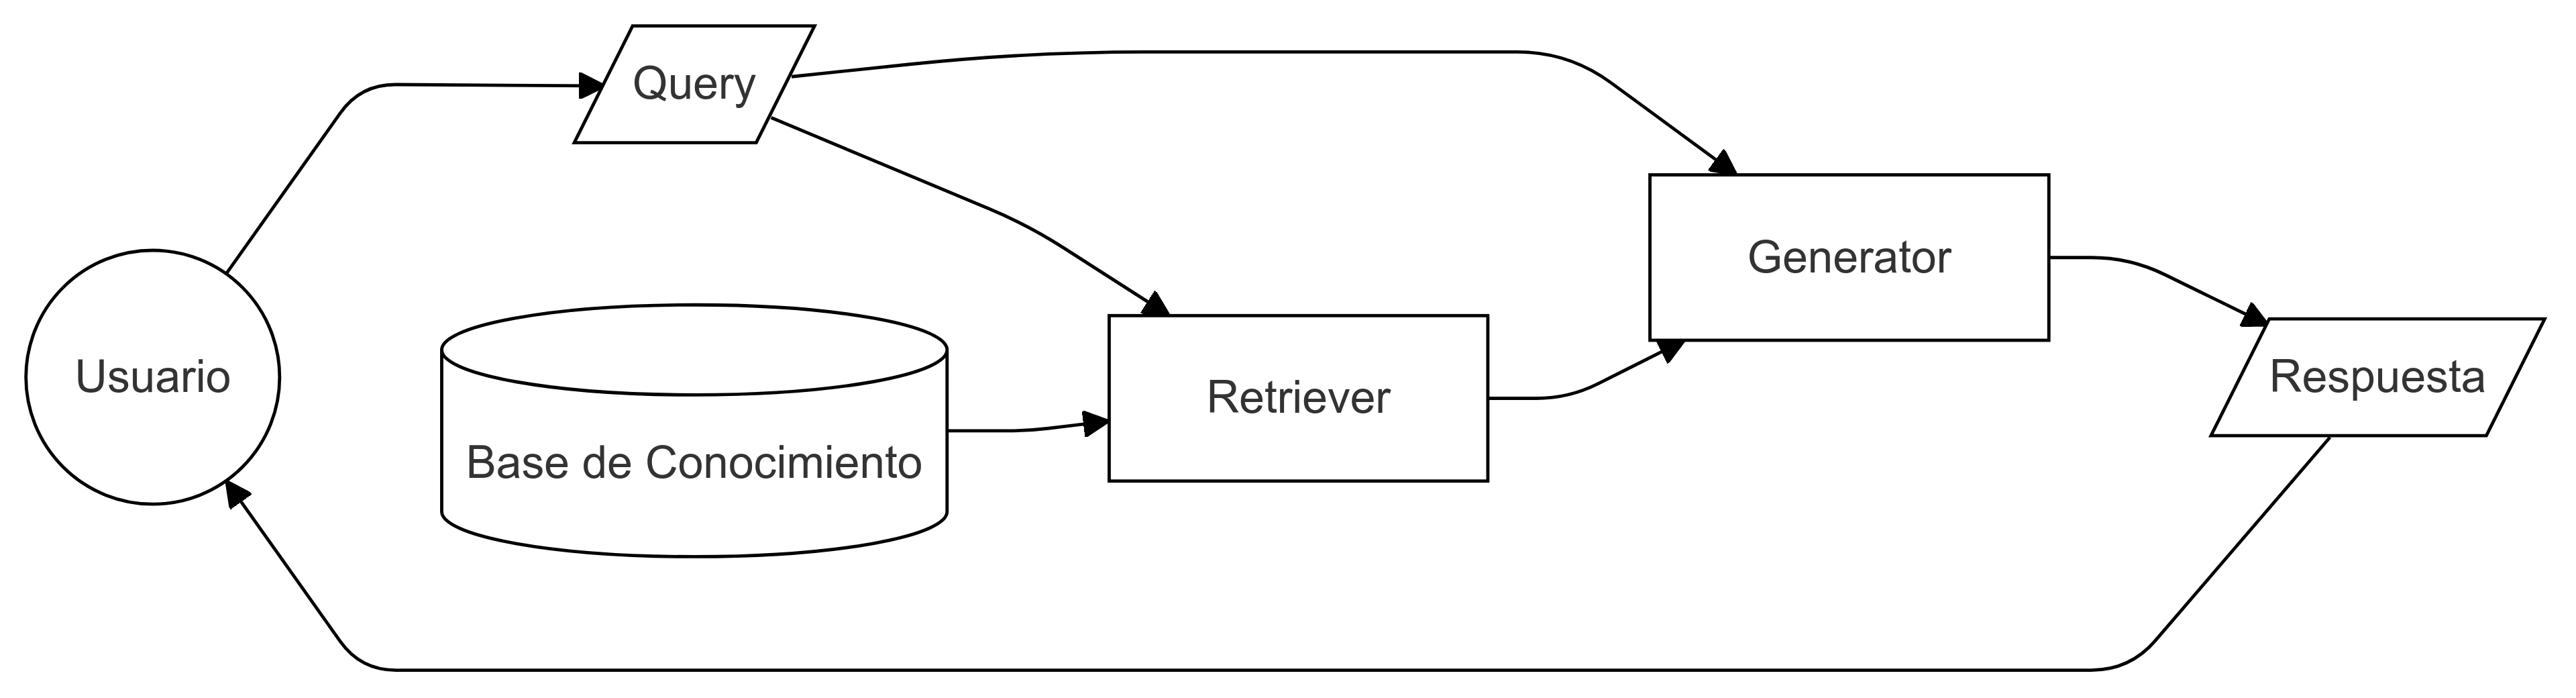
\includegraphics[width=0.8\textwidth]{figuras/rag-flow.png}
  \caption{Flujo de información en un sistema RAG}
  \label{fig:rag-flow}
\end{figure}

El proceso de generación sigue tres pasos fundamentales:

\begin{enumerate}
  \item \textbf{Recuperación de documentos relevantes}: El sistema vectoriza la consulta del usuario y busca en la base de conocimiento utilizando índices semánticos para encontrar documentos relacionados.

  \item \textbf{Análisis y ranking de documentos}: Se evalúa la relevancia de los documentos recuperados considerando su similitud semántica con la consulta y la confiabilidad de las fuentes.

  \item \textbf{Generación de respuestas}: El \gls{llm} integra el conocimiento recuperado con el contexto de la consulta para producir una respuesta coherente y precisa.
\end{enumerate}

\subsection{Aplicaciones y Ventajas de RAG en Educación}

Los sistemas \gls{rag} ofrecen beneficios significativos para aplicaciones educativas, especialmente en la enseñanza de idiomas. Las ventajas principales incluyen:

\begin{itemize}
  \item \textbf{Precisión y Confiabilidad:} Mayor precisión en la información proporcionada al combinar conocimiento estructurado con la flexibilidad de los \gls{llm}, reduciendo \gls{hallucinations} y respuestas incorrectas al anclar la generación en fuentes confiables.

  \item \textbf{Trazabilidad y Verificabilidad:} Capacidad de citar fuentes y materiales relevantes, proporcionando referencias verificables para el contenido educativo.

  \item \textbf{Adaptabilidad y Actualización:} estos sistemas ofrecen adaptabilidad a diferentes dominios mediante la actualización de la base de conocimiento. Esto permite una actualización dinámica del contenido sin necesidad de reentrenar el modelo completo. Además, facilita la personalización del contenido educativo mediante la selección específica de fuentes relevantes para cada estudiante.
\end{itemize}

\section{Aprendizaje por Refuerzo}

\subsection{Fundamentos Teóricos del RL}

El Aprendizaje por Refuerzo proporciona un marco matemático ideal para la personalización del aprendizaje de idiomas. Basado en \gls{mdp}, permite modelar el proceso de aprendizaje como una serie de decisiones secuenciales, donde el sistema debe seleccionar las actividades y contenidos más apropiados según el nivel y progreso del estudiante \cite{williams2017educational}.

En nuestro contexto, el estado representa el perfil actual del estudiante, incluyendo su dominio del idioma en diferentes áreas (comprensión, producción, vocabulario, gramática), mientras que las acciones corresponden a las diferentes intervenciones pedagógicas disponibles.

\subsection{Proximal Policy Optimization (PPO)}

PPO \cite{schulman2017proximal} es un algoritmo de \gls{rl} que destaca por su estabilidad y eficiencia en el aprendizaje de políticas. En nuestro sistema de aprendizaje de idiomas, PPO se utiliza para optimizar la selección de actividades y la adaptación del contenido.


\subsubsection{Formulación Matemática}
El objetivo de PPO es maximizar la siguiente función objetivo:

\begin{equation}
  L^{CLIP}(\theta) = \hat{\mathbb{E}}_t[\min(r_t(\theta)\hat{A}_t, \text{clip}(r_t(\theta), 1-\epsilon, 1+\epsilon)\hat{A}_t)]
\end{equation}

Donde:

\begin{itemize}
  \item $r_t(\theta)$ es el ratio de probabilidades entre la política nueva y antigua
  \item $\hat{A}_t$ es la estimación de la ventaja
  \item $\epsilon$ es el parámetro de clipping (típicamente 0.2)
\end{itemize}

\begin{algorithm}[H]
  \label{alg2}
  \SetAlgoLined
  \medskip
  \begin{enumerate}
    \item Inicializar los parámetros de la política $\theta$ y el valor función $\phi$
    \item Para cada iteración:
          \begin{enumerate}
            \item Recopilar conjunto de trayectorias $\mathcal{D}_k = \{\tau_i\}$ ejecutando la política $\pi_\theta$ en el entorno
            \item Calcular ventajas estimadas $\hat{A}_t$ usando función de valor actual $V_\phi$
            \item Para cada época de optimización:
                  \begin{enumerate}
                    \item Calcular ratio de probabilidad $r_t(\theta) = \frac{\pi_\theta(a_t|s_t)}{\pi_{\theta_{old}}(a_t|s_t)}$
                    \item Calcular pérdida recortada:
                          $$L^{CLIP}(\theta) = \hat{\mathbb{E}}_t[\min(r_t(\theta)\hat{A}_t, \text{clip}(r_t(\theta), 1-\epsilon, 1+\epsilon)\hat{A}_t)]$$
                    \item Actualizar $\theta$ minimizando $-L^{CLIP}(\theta)$ usando descenso de gradiente
                    \item Actualizar función de valor $\phi$ minimizando error cuadrático medio
                  \end{enumerate}
            \item Actualizar $\theta_{old} \leftarrow \theta$
          \end{enumerate}
    \item Devolver la política optimizada $\pi_\theta$
  \end{enumerate}
  \caption{Algoritmo \textit{Proximal Policy Optimization} (PPO)}
\end{algorithm}

\subsubsection{Aplicación en el Sistema}

En nuestro contexto educativo:

\begin{itemize}
  \item \textbf{Estado ($\mathcal{S}$):} Representa el perfil actual del estudiante.
        \begin{equation}\label{eq:state}
          \mathcal{S} = \{\text{vocabulario\_nivel} = \text{B1}, \text{gramática\_nivel} = \text{A2}, \text{pronunciación\_nivel} = \text{B2}\}
        \end{equation}

  \item \textbf{Acciones ($\mathcal{A}$):} Selección de actividades y sus parámetros.
        \begin{equation}\label{eq:actions}
          \mathcal{A} = \{\text{ejercicio\_gramática\_A2}, \text{práctica\_vocabulario\_B1}, \text{diálogo\_pronunciación\_B2}\}
        \end{equation}

  \item \textbf{Recompensa ($\mathcal{R}$):} Evalúa el éxito de cada acción. Por ejemplo, si después de un ejercicio de gramática el estudiante mejora su precisión del 60\% al 80\%, $\mathcal{R} = +20$

  \item \textbf{Política ($\pi$):} Determina qué acción tomar en cada estado. Por ejemplo, si el estudiante muestra consistentemente errores en gramática, $\pi$ seleccionará más ejercicios gramaticales
\end{itemize}

\subsubsection{Sistema de Recompensas}

La \gls{reward-function} se diseña específicamente para el aprendizaje de idiomas, evaluando el desempeño y proporcionando retroalimentación a través de múltiples dimensiones:

\begin{itemize}
  \item \textbf{Recompensas inmediatas:} Incluyen la precisión en las respuestas y ejercicios, mejora en la pronunciación y fluidez, uso correcto de estructuras gramaticales, y la adquisición y retención de vocabulario.

  \item \textbf{Recompensas a largo plazo:} Consideran el progreso sostenido en múltiples dimensiones lingüísticas, la mejora en la competencia comunicativa general, y la retención y aplicación de conocimientos previos.

  \item \textbf{Ajustes dinámicos:} Comprenden la calibración automática de pesos de recompensa, adaptación a diferentes estilos y velocidades de aprendizaje, y el balanceo entre diferentes competencias lingüísticas.
\end{itemize}

\subsection{Evaluación de Políticas de Aprendizaje}

La evaluación de la \gls{policy} en sistemas de aprendizaje de idiomas requiere un enfoque multidimensional que considere tanto aspectos cuantitativos como cualitativos. \cite{williams2017educational} propone un marco de evaluación que examina:

\begin{itemize}
  \item \textbf{Progreso en competencias lingüísticas específicas:} Incluye la mejora en precisión gramatical y uso de estructuras, expansión del vocabulario activo y pasivo, desarrollo de fluidez y pronunciación, y avance en comprensión auditiva y lectora.

  \item \textbf{Efectividad de la personalización:} Abarca la adaptación a estilos individuales de aprendizaje, respuesta a patrones de error específicos, ajuste dinámico del nivel de dificultad y personalización de contenido temático.

  \item \textbf{Eficiencia en el tiempo de aprendizaje:} Considera la tasa de adquisición de nuevos conceptos, reducción en tiempo de dominio de habilidades, optimización de intervalos de repaso y minimización de redundancia en ejercicios.

  \item \textbf{Engagement y retención del estudiante:} Evalúa los niveles de participación activa, tasas de completación de actividades, persistencia en el programa de aprendizaje y satisfacción reportada por el estudiante.
\end{itemize}

La evaluación se realiza mediante métricas cuantitativas específicas:

\begin{equation}
  \text{Efectividad} = \frac{\text{Objetivos Alcanzados}}{\text{Tiempo Invertido}} \times \text{Factor de Dificultad}
\end{equation}

\begin{equation}
  \text{Índice de Personalización} = \frac{\sum_{i=1}^{n} \text{Adaptaciones Exitosas}_i}{n} \times \text{Tasa de Progreso}
\end{equation}

Estas métricas se complementan con análisis cualitativo continuo y retroalimentación directa de los estudiantes para asegurar una evaluación holística de la \gls{policy}.


\section{Tecnologías de Procesamiento de Voz}

El procesamiento de voz en sistemas de aprendizaje de idiomas involucra dos procesos fundamentales: el reconocimiento automático del habla (\gls{stt}) y la síntesis de voz (\gls{tts}). Estos procesos representan transformaciones complementarias entre el dominio acústico y el lingüístico.

\subsection{Reconocimiento Automático del Habla (STT)}

El proceso de STT transforma señales acústicas en texto, involucrando múltiples etapas de procesamiento y análisis. Este proceso se fundamenta en principios de procesamiento de señales y modelos probabilísticos del lenguaje \cite{graves2013speech}.

\subsubsection{Procesamiento de la Señal Acústica}

\begin{itemize}
  \item \textbf{Preprocesamiento Acústico:} La señal de audio cruda se somete a técnicas de reducción de ruido, normalización de amplitud y segmentación en tramas. Este proceso mejora la calidad de la señal y la prepara para el análisis posterior.

  \item \textbf{Extracción de Características:} Se extraen representaciones espectrales como coeficientes \gls{mfcc}, que capturan las características acústicas relevantes para el reconocimiento del habla.

  \item \textbf{Normalización de Características:} Las características extraídas se normalizan para reducir variaciones no lingüísticas como diferencias en el volumen o el canal de grabación.
\end{itemize}

\subsubsection{Proceso de Reconocimiento}

\begin{itemize}
  \item \textbf{Modelado Acústico:} Se analiza la relación entre las características acústicas y las unidades fonéticas del habla, considerando variaciones en pronunciación y contexto fonético.

  \item \textbf{Modelado del Lenguaje:} Se incorpora conocimiento sobre la estructura del lenguaje, incluyendo probabilidades de secuencias de palabras y restricciones gramaticales.

  \item \textbf{Decodificación:} Se combina la información acústica y lingüística para determinar la secuencia más probable de palabras, utilizando algoritmos de búsqueda como \gls{viterbi} o \gls{beam-search}.
\end{itemize}

\subsection{Síntesis de Voz (TTS)}

La síntesis de voz realiza la transformación inversa, convirtiendo texto en señales de habla mediante un proceso que combina análisis lingüístico y generación de señales acústicas \cite{taylor2009text}.


\subsubsection{Procesamiento Lingüístico}

\begin{itemize}
  \item \textbf{Análisis de Texto:} Se procesa el texto de entrada para identificar su estructura lingüística, incluyendo tokenización, normalización y análisis sintáctico.

  \item \textbf{Conversión Grafema-Fonema:} Se transforma el texto escrito en su representación fonética, considerando reglas de pronunciación y excepciones específicas del idioma.

  \item \textbf{Análisis Prosódico:} Se determinan patrones de entonación, duración y énfasis basados en la estructura sintáctica y semántica del texto.
\end{itemize}

\subsubsection{Generación de Voz}

\begin{itemize}
  \item \textbf{Modelado Prosódico:} Se generan patrones detallados de pitch, duración y energía para cada fonema, considerando el contexto lingüístico y emocional.

  \item \textbf{Generación de Características Acústicas:} Se producen representaciones espectrales intermedias que codifican las propiedades acústicas deseadas del habla.

  \item \textbf{Síntesis de Forma de Onda:} Se genera la señal de audio final mediante técnicas de síntesis que pueden ser concatenativas, paramétricas o basadas en modelos neuronales.
\end{itemize}

\subsection{Integración en Sistemas de Aprendizaje}

La combinación de STT y TTS en sistemas educativos permite crear ciclos completos de interacción oral:

\begin{itemize}
  \item \textbf{Ciclo de Retroalimentación:} El sistema puede generar ejemplos de pronunciación (TTS), analizar la producción del estudiante (STT) y proporcionar retroalimentación específica.

  \item \textbf{Análisis de Precisión:} La comparación entre la transcripción del habla del estudiante y el texto objetivo permite evaluar la precisión de pronunciación y fluidez.

  \item \textbf{Adaptación Dinámica:} Los resultados del análisis permiten ajustar parámetros como velocidad del habla, complejidad del contenido y umbral de aceptación de pronunciación.
\end{itemize}